%slide relative ad introdurre gli elementi di XML Schema Definition (XSD) 

%frame 01
\begin{frame}
	\frametitle{Elementi per la definizione degli schemi xml}
	\framesubtitle{principi XML Schema Definition}
	\addtocounter{nframe}{1}

	\begin{block}{Cos'è uno schema XML}
		Uno schema XML è un documento XML standard che descrive come deve essere realizzato un altro documento XML.
		\\ Ci riferiamo a questa tecnologia con l'acronimo XSD.
	\end{block}

	\begin{block}{A cosa serve uno Schema XML}
		I documenti XSD sono usati per validare documenti XML.
		\\ Tuttavia un documento XSD viene realizzato tramite l'uso di un vocabolario predefinito riferibile attraverso un namespace con URI standard.
	\end{block}

\end{frame}

%frame 02
\begin{frame}
	\frametitle{Elementi per la definizione degli schemi xml}
	\framesubtitle{principi XSD}
	\addtocounter{nframe}{1}

	\begin{block}{XSD Schema}
		Il termine XSD o XML Schema denota un documento XML che descrive e valida la struttura e il contenuto di un altro documento XML.
	\end{block}

	\begin{block}{XSD Schema}
		\textbf{Dichiarazione del documento (declaration) e istanza del documento (instance).}
	\end{block}

\end{frame}

%frame 03
\begin{frame}
	\frametitle{Elementi per la definizione degli schemi xml}
	\framesubtitle{principi XSD}
	\addtocounter{nframe}{1}

	\begin{block}{XSD elemento root}
		L'elemento radice di uno schema XSD è sempre l'elemento ``\texttt{<schema>}''.
		\\ Tutte le definizione devono seguire quindi l'elemento ``\texttt{<schema>}''.
	\end{block}

	\begin{block}{XSD Schema}
		Tutti gli elementi e gli attributi dello schema sono dichiarati all'interno del namespace ``\texttt{http://www.w3.org/2001/XMLSchema.}''.
		\\ Tutti i documenti XSD contengono la dichiarazione a questo namespace con prefisso convenzionale \textbf{xsd} oppoure \textbf{xs}.
	\end{block}

\end{frame}

\begin{frame}
	\frametitle{Elementi per la definizione degli schemi xml}
	\framesubtitle{principi XSD}
	\addtocounter{nframe}{1}

	\begin{block}{XSD componenti di base}
		I componenti di base di uno Schema XSD sono le dichiarazioni degli elementi e le dichiarazioni degli attributi.
	\end{block}

	\begin{block}{XSD Schema}
		\textbf{Le dichiarazioni più complesse si poggiano su queste unità: elementi e attributi.}
	\end{block}

\end{frame}

\begin{frame}
	\frametitle{Elementi per la definizione degli schemi xml}
	\framesubtitle{principi XSD}
	\addtocounter{nframe}{1}

	\begin{block}{XSD dichiarazioni}
		Scrivere un pezzo di codice XSD per descrivere e validare un elemento per un documento XML è detto \textit{element declaration}.
	\end{block}

	\begin{block}{XSD dichiarazioni di base}
		XSD permette di dichiarare elementi, attributi e di specificare il numero di figli, le occorrenze, l'ordine di apparizione, e i tipi di dati del content model.
	\end{block}

\end{frame}


\begin{frame}
	\frametitle{Elementi per la definizione degli schemi xml}
	\framesubtitle{principi XSD}
	\addtocounter{nframe}{1}

	\begin{block}{Element Types: simple and complex}
		La dichiarazione di un elemento può avere un tipo semplice (\textit{simple type}) oppure un tipo complesso (\textit{complex type}) a seconda della sua struttura e del suo contenuto.


	\end{block}

	\begin{block}{Simple Type e Complex Type}
		La dichiarazione di un elemento ha un tipo semplice se non possiede \textbf{né figli né attributi}.
		\\ La dichiarazione di un elemento ha un tipo complesso in tutti gli altri casi.
	\end{block}

\end{frame}


%frame 04
\begin{frame}
	\frametitle{Elementi per la definizione degli schemi xml}
	\framesubtitle{principi XSD}
	\addtocounter{nframe}{1}

	%\defverbatim{\xsdfirst}{%
	%\begin{tiny}
	%\begin{verbatim}
	%    <xsd:schema xmlns:xsd="http://www.w3.org/2001/XMLSchema">
	%        <xsd:element name="text"/>
	%    </xsd:schema>
	%\end{verbatim}
	%    \end{tiny}
	%   }

	%  \defverbatim{\xmlfirst}{%
	% \begin{tiny}
	%\begin{verbatim}
	%         <text>Il primo documento XML Validato</text>
	% \end{verbatim}
	% \end{tiny}
	% }


	\begin{block}{XSD esempio}
		% {\xsdfirst}
		\texttt{<xsd:schema xmlns:xsd=``http://www.w3.org/2001/XMLSchema''>}
		\\\texttt{<xsd:element name=``text''/>}
		\\\texttt{</xsd:schema>}
	\end{block}

	\begin{block}{XSD esempio elemento di tipo semplice}
		% {\xsdfirst}
		\texttt{<text>Il primo documento XML Validato</text>}
	\end{block}



\end{frame}

\begin{frame}
	\frametitle{Elementi per la definizione degli schemi xml}
	\framesubtitle{principi XSD}
	\addtocounter{nframe}{1}

	\begin{block}{XML XSD esempio}
		Il documento XML istanza dello schema XSD per essere valido deve contenere un elemento radice.
		Validare il documento XML con il relativo XSD con XMLlint.

	\end{block}

	\begin{block}{XMLlint}
		\texttt{xmllint xmlfirst.xml --schema ../schema/xsd/xsdfirst.xsd}
	\end{block}


\end{frame}

\begin{frame}
	\frametitle{Elementi per la definizione degli schemi xml}
	\framesubtitle{principi XSD}
	\addtocounter{nframe}{1}

	\begin{block}{Element Complex Types: esempio}

		%If an element contains child elements or attributes, it has a complex type.
		\texttt{
			<xsd:schema xmlns:xsd=``http://www.w3.org/2001/XMLSchema''>
			<xsd:element name=``Employee''>
			<xsd:complexType>
			<xsd:attribute name=``FirstName''/>
			</xsd:complexType>
			</xsd:element>
			</xsd:schema>
		}
	\end{block}

	\begin{block}{Element Complex Types: esempio}
		Il documento XML istanza dello schema:
		\\\texttt{<Employee FirstName="Jacob"/>}
	\end{block}

\end{frame}

\begin{frame}
	\frametitle{Elementi per la definizione degli schemi xml}
	\framesubtitle{principi XSD}
	\addtocounter{nframe}{1}

	\begin{block}{Complex Types}
		Alla base dello standard XSD ci sono le dichiarazioni degli elementi e degli attributi, ad un livello di astrazione più alto ci sono i types e i groups.
		\\ A complex type can have attributes, child elements or both. Here is another example that shows a complex type having child elements.

	\end{block}

	\begin{block}{Element Complex Types: Esempio Elemento con Figlio}
		\texttt{
			<xsd:schema xmlns:xsd=``http://www.w3.org/2001/XMLSchema''>
			<xsd:element name=``text''>
			<xsd:complexType>
			<xsd:sequence>
			<xsd:element name=``body''/>
			</xsd:sequence>
			</xsd:complexType>
			</xsd:element>
			</xsd:schema>}
	\end{block}

\end{frame}

\begin{frame}
	\frametitle{Elementi per la definizione degli schemi xml}
	\framesubtitle{principi XSD}
	\addtocounter{nframe}{1}

	\begin{block}{Espressività dell'XSD}

		\begin{itemize}
			\item Attribute Group, Element Group
			\item Order Indicators: all, sequence, choice
			\item Occurrence Indicators: minOccurs and maxOccurrs
			\item Annotation (utili per documentare le dichiarazioni)
		\end{itemize}

	\end{block}

	\begin{block}{Espressività dell'XSD}
		\begin{itemize}
			\item Data types: Built-in
			\item FACETS per una validazione oculata dei valori (elemento o un attributo).
			\item Restriction on base attribute
			\item Numeric e String Data Type
			\item Pattern facet
		\end{itemize}

	\end{block}

\end{frame}


\begin{frame}
	\frametitle{Elementi per la definizione degli schemi xml}
	\framesubtitle{principi XSD}
	\addtocounter{nframe}{1}

	\begin{block}{Element Declaration}

		An XSD element declaration represents an element in the XML instance document
		An element is said to have a Simple Type if it does not have any attributes and does not have child elements.
	\end{block}

	\begin{block}{Element Declaration: Istanza XML }
		\texttt{<p>il contentuto testuale di un paragrafo</p>}
	\end{block}

\end{frame}


%% An XSD schema may contain Global and Local element declarations.

\begin{frame}
	\frametitle{Elementi per la definizione degli schemi xml}
	\framesubtitle{principi XSD}
	\addtocounter{nframe}{1}

	\begin{block}{Global and Local element declaration}
		The advantage of using a global element declaration is that it can be reused (referred) at other locations from within the same schema.
		\\ When you have a global element declaration, you can refer it in multiple locations in your schema (level of reusability).
	\end{block}

	\begin{block}{Global element declaration: esempio}
		\texttt{<xsd:schema xmlns:xsd=``http://www.w3.org/2001/XMLSchema">
			<xsd:element name=``body''>
			<xsd:complexType>
			<xsd:attribute name=``lang''/>
			<xsd:attribute name=``type''/>
			</xsd:complexType>
			</xsd:element>
			<xsd:element name=``text''>
			<xsd:complexType>
			<xsd:all>
			<xsd:element ref=``body''/>
			</xsd:all>
			</xsd:complexType>
			</xsd:element>
			</xsd:schema>}
	\end{block}

\end{frame}

\begin{frame}
	\frametitle{Elementi per la definizione degli schemi xml}
	\framesubtitle{principi XSD}
	\addtocounter{nframe}{1}

	\begin{block}{Group declaration}
		Commonly used attributes and elements can be grouped together into Attribute Groups and Element Groups. You can then refer to such a group at multiple locations in your schema definition. Attribute groups and Element groups provide a certain level of reusability.
	\end{block}

\end{frame}



\begin{frame}
	\frametitle{Elementi per la definizione degli schemi xml}
	\framesubtitle{principi XSD}
	\addtocounter{nframe}{1}


	\begin{block}{Global element declaration: esempio}
		\texttt{<xsd:group name=``fileDesc''>
			<xsd:sequence>
			<xsd:element name=``titleStmt''/>
			<xsd:element name=``publicationStmt''/>
			<xsd:element name=``sourceDesc''/>
			</xsd:sequence>
		}
	\end{block}

	\begin{block}{Global element declaration: esempio}
		\texttt{<xsd:group ref=``fileDesc''/>
		}
	\end{block}



\end{frame}

\begin{frame}
	\frametitle{Elementi per la definizione degli schemi xml}
	\framesubtitle{principi XSD}
	\addtocounter{nframe}{1}

	\begin{block}{Element Declaration: Attributi}
		Attributi della dichiarazione di elementi: The only mandatory attribute that an element declaration should take is the ``name'' attribute.
	\end{block}

	\begin{block}{Element Declaration: Attributi - Esempio}
		\texttt{<xsd:element name=``TEI''/> }
	\end{block}

\end{frame}

\begin{frame}
	\frametitle{Elementi per la definizione degli schemi xml}
	\framesubtitle{principi XSD}
	\addtocounter{nframe}{1}

	\begin{block}{Element declaration: lista Attributi}
		\begin{itemize}
			\item \textbf{name} (\textit{g-l})
		\end{itemize}

		%\begin{itemize}
		%\item \textbf{name} (\textit{g-l}) the only mandatory attribute (give meaningful names to the elements)
		%\item type (g-l) adds data type related validations to the declaration of an element (XSD has buint-in data types)
		%\item id (g-l) uniquely identifies the given element (non ha effetti sull'istanza XML
		%\item default (g-l) specify the default value of an element (solo de l'elemento opzionale)
		%\item fixed (g-l) valore di un elemento predefinito (``fixed'' and ``default'' are mutually exclusive)
		%\item nillable (g-l) indica che l'elemento è vuoto (xsd:nil nell'istanza XML del documento)
		%\item block (g-l) It is used to control substitution (4 different vales, namely: substitution, extension restriction and #all)
		%\end{itemize}

	\end{block}

\end{frame}


\begin{frame}
	\frametitle{Elementi per la definizione degli schemi xml}
	\framesubtitle{principi XSD}
	\addtocounter{nframe}{1}

	\begin{block}{Element declaration: lista Attributi (cont.)}

		\begin{itemize}
			\item \textbf{final} (\textit{g}) limits
		\end{itemize}
		%\item final (g) limits the declaration of substitution groups in schemas (can take values: #all, restriction and extension.)
		%\item abstract (g) When an element is declared as abstract, it cannot be instantiated (force an element substitution)
		%\item substitutionGroup (g) is highly extensible (could easily add new types derived) esempio SG
		%\item minOccurs (l) control the occurrence of the elements: minimum number of times the element should appear in the XML instance (minOccurs=0 -> Optional).
		%\item maxOccurs (l) control the occurrence of the elements: The maximum number of times the element can appear within its parent.
		%\item ref (l) Refer to other elements declared globally in the same schema (certain level of reusability)
		%\item form (l) specifies whether the element needs to be qualified with a namespace prefix (be ``qualified'' or ``unqualified'')


	\end{block}

\end{frame}


\begin{frame}
	\frametitle{Elementi per la definizione degli schemi xml}
	\framesubtitle{principi XSD}
	\addtocounter{nframe}{1}

	\begin{block}{Element declaration: Attributi - Esempio }

		\texttt{
			<xsd:element name=``body''>
			<xsd:complexType>
			<xsd:sequence maxOccurs=``unbounded''>
			<xsd:element ref=``div''/>
			</xsd:sequence>
			</xsd:complexType>
			</xsd:element>
		}

	\end{block}


	\begin{block}{Element declaration: Attributi - Esempio }

		\texttt{
			<xsd:element name=``div'' type=``divType'' />
		}
		\texttt{
			<xsd:complexType name=``divType''>
			[...]
			</xsd:complexType>
		}

	\end{block}

\end{frame}






% Attribute Declaration
% simple example
% <xsd:schema xmlns:xsd="http://www.w3.org/2001/XMLSchema">
%   <xsd:element name="Employee">
%     <xsd:complexType>
%       <xsd:attribute name="status" />
%     </xsd:complexType>
%   </xsd:element>
% </xsd:schema>



\begin{frame}
	\frametitle{Elementi per la definizione degli schemi xml}
	\framesubtitle{principi XSD}
	\addtocounter{nframe}{1}

	\begin{block}{Attribute declaration:}
		An attribute is declared with <xsd:attribute> element. The only mandatory attribute of an attribute declaration is ``name''.
		\\ When an attribute is declared right under the ``<xsd:schema>'' element, it is called global attribute declaration. When it is declared within a Complex Type, it is called Local attribute declaration.
	\end{block}


	\begin{block}{Attribute declaration}

		\texttt{
			<xsd:attribute name=``Name'' type=``xsd:string''/>
		}

	\end{block}
	\textit{Qualsiasi dichiarazione di attributo per essere effettivamente utile deve essere fatta all'interno di una dichiarazione di elemento}

\end{frame}



% tabella con gli attributi nella dichiarazione degli attributi
% "attributes of an attribute declaration"

\begin{frame}
	\frametitle{Elementi per la definizione degli schemi xml}
	\framesubtitle{principi XSD}
	\addtocounter{nframe}{1}

	\begin{block}{Attribute declaration: Attributi}
		\begin{itemize}
			\item \textbf{name} (\textit{g-l}) the name of the attribute as it should appear in the XML instance (Mandatory)
			\item id (g-l) used by the schema processor to uniquely identify the XSD components within a given schema
			\item type (g-l) associates a data type with an attribute (facilitates validation on the value). make sure that only valid values are accepted
		\end{itemize}

	\end{block}


\end{frame}


\begin{frame}
	\frametitle{Elementi per la definizione degli schemi xml}
	\framesubtitle{principi XSD}
	\addtocounter{nframe}{1}

	\begin{block}{Attribute declaration: Attributi (cont.)}
		\begin{itemize}
			\item \textbf{default} (\textit{g-l}) The default attribute assigns a default value to an attribute declaration (solo se l'attributo non è presente)
			\item fixed (g-l) It prevents the attribute from taking any value other than the pre-defined one.
			\item ref (l) A globally declared attribute can be inserted into a complex type by using the ``ref'' attribute.
			\item use (l) specifies whether the attribute is optional or mandatory (values optional or required, prohibited).
			\item form (l) specifies whether the attribute needs to be qualified by a namespace prefix or not, in the XML instance. (può assumere due valori: qualified e unqualified)
		\end{itemize}

	\end{block}


\end{frame}

\begin{frame}
	\frametitle{Elementi per la definizione degli schemi xml}
	\framesubtitle{principi XSD}
	\addtocounter{nframe}{1}

	\begin{block}{Attribute declaration: Esempio (global)}

		\texttt{
			<xsd:schema xmlns:xsd=``http://www.w3.org/2001/XMLSchema''>
			<xsd:attribute name=``analysis'' />
			<!-- -->
			<xsd:element name=``word''>
			<xsd:complexType>
			<xsd:attribute ref=``analysis''/>
			</xsd:complexType>
			</xsd:element>
			</xsd:schema>
		}

	\end{block}

	\textit{Global attribute declarations are useful when an attribute is declared with several validations}


\end{frame}



%% Esempio da img GlobalAttribute
%% global attribute declarations provide some sort of re-usability.

%% esempio type:
% <xsd:schema xmlns:xsd="http://www.w3.org/2001/XMLSchema">
%   <xsd:element name="Employee">
%     <xsd:complexType>
%       <xsd:attribute name="Age" type="xsd:positiveInteger"/>
%     </xsd:complexType>
%   </xsd:element>
% </xsd:schema>

%% Attribute Groups
% Attribute Groups provide a convenient means to reuse attribute declarations in multiple complex types. Attribute Groups provide a better level of reusability by grouping one or more attribute declarations into a named group. By using an attribute group, you can avoid this repetition of code. Chain of attribute group hierarchies.

\begin{frame}
	\frametitle{Elementi per la definizione degli schemi xml}
	\framesubtitle{principi XSD}
	\addtocounter{nframe}{1}

	\begin{block}{Attribute declaration: Attribute Groups}
		Attribute Groups provide a convenient means to reuse attribute declarations in multiple complex types. Attribute Groups provide a better level of reusability by grouping one or more attribute declarations into a named group. By using an attribute group, you can avoid this repetition of code. Chain of attribute group hierarchies.
	\end{block}



\end{frame}



\begin{frame}
	\frametitle{Elementi per la definizione degli schemi xml}
	\framesubtitle{principi XSD}
	\addtocounter{nframe}{1}

	\begin{block}{Attribute declaration: Esempio (global)}
		\texttt{
			<xsd:schema xmlns:xsd=``http://www.w3.org/2001/XMLSchema''>
			<xsd:attributeGroup name=``EmpAttributes''>
			<!-- Declaration of attribute ``name'' -->
			<xsd:attribute name=``name''>
			<xsd:simpleType>
			<xsd:restriction base=``xsd:string''>
			<xsd:maxLength value=``20''/>
			</xsd:restriction>
			</xsd:simpleType>
			</xsd:attribute>
			<!-- Declaration of attribute ``department'' -->
			<xsd:attribute name=``department''>
			<xsd:simpleType>
			<xsd:restriction base=``xsd:string''>
			<xsd:length value=``2''/>
			</xsd:restriction>
			</xsd:simpleType>
			</xsd:attribute>
			</xsd:attributeGroup>
			[...]
		}
	\end{block}

	\textit{Global attribute declarations are useful when an attribute is declared with several validations}


\end{frame}


\begin{frame}
	\frametitle{Elementi per la definizione degli schemi xml}
	\framesubtitle{principi XSD}
	\addtocounter{nframe}{1}

	\begin{block}{Attribute declaration: Esempio (global)}
		\texttt{
			[...]
			<!-- Declaration of root element ``Employees'' -->
			<xsd:element name=``Employees''>
			<xsd:complexType>
			<xsd:sequence>
			<!-- Declaration of ``Manager'' element -->
			<xsd:element name=``Manager''>
			<xsd:complexType>
			<xsd:attributeGroup ref=``EmpAttributes''/>
			</xsd:complexType>
			</xsd:element>
			<!-- Declaration of ``department'' element -->
			<xsd:element name=``TechLead''>
			<xsd:complexType>
			<xsd:attributeGroup ref=``EmpAttributes''/>
			</xsd:complexType>
			</xsd:element>
			</xsd:sequence>
			</xsd:complexType>
			</xsd:element>
			</xsd:schema>
		}
	\end{block}

	\textit{Global attribute declarations are useful when an attribute is declared with several validations}


\end{frame}




%% Data type

\begin{frame}
	\frametitle{Elementi per la definizione degli schemi xml}
	\framesubtitle{principi XSD}
	\addtocounter{nframe}{1}

	\begin{block}{XSD Data Type}

		Programming languages use data types to make sure that correct values are stored to variables and correct operations are done using those variables.
	\end{block}

	\begin{block}{XSD Data Type}
		When you associate a variable to a data type you are basically restricting the values that the variable can store and restricting the permissible operations on them.
	\end{block}

\end{frame}

\begin{frame}
	\frametitle{Elementi per la definizione degli schemi xml}
	\framesubtitle{principi XSD}
	\addtocounter{nframe}{1}

	\begin{block}{XSD Data Type: esempio -  dichiarazione}
		\texttt{
			<xsd:schema xmlns:xsd=``http://www.w3.org/2001/XMLSchema''>
			<xsd:element name=``div''>
			<xsd:complexType>
			<xsd:attribute name=``type'' />
			<xsd:attribute name=``n'' type=``xsd:integer''/>
			</xsd:complexType>
			</xsd:element>
			</xsd:schema>
		}


	\end{block}

	\begin{block}{XSD Data Type: esempio - istanza}
		\texttt{<div type="chapter" n="1" />'} \textit{(corretto)}
		\\\texttt{<div type="chapter" n="uno" />'} \textit{(errato)}

	\end{block}



\end{frame}

\begin{frame}
	\frametitle{Elementi per la definizione degli schemi xml}
	\framesubtitle{principi XSD}
	\addtocounter{nframe}{1}

	\begin{block}{XSD Data Type}


		XSD supports a number of different data types to describe and validate almost all values that we might need to work with.
		It supports deriving new data types from the built-in data types


	\end{block}

	\begin{block}{XSD Data Type}
		Data types help describe a certain piece of data more accurately and help validate them more efficiently.
		\\ XSD supports almost fifty data types. They can be divided into Primitive Data Types, Derived Data Types

	\end{block}



\end{frame}

\begin{frame}
	\frametitle{Elementi per la definizione degli schemi xml}
	\framesubtitle{principi XSD}
	\addtocounter{nframe}{1}

	\begin{block}{Primitive Data Types}

		Primitive Data Types are base data types from which other data types are derived.
		\\XSD has nineteen primitive data types

	\end{block}

	\begin{block}{Primiteive Data Types}

		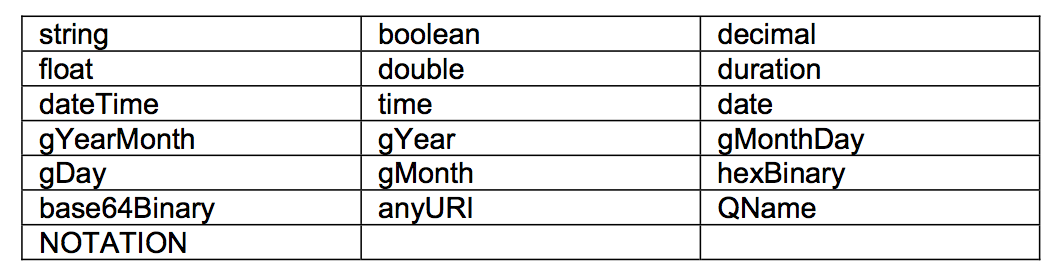
\includegraphics[width=.95\textwidth]{imgs/TabellaDataTypeXSD.png}

	\end{block}

\end{frame}

\begin{frame}
	\frametitle{Elementi per la definizione degli schemi xml}
	\framesubtitle{principi XSD}
	\addtocounter{nframe}{1}

	\begin{block}{Primitive Data Types}


		Primitive Data Types are the base data types of XSD. This means that they themselves have not been derived from another type.


	\end{block}

	\begin{block}{Derived Data Types}

		These are Data Types derived directly or indirectly from Primitive Data Types.

	\end{block}

\end{frame}


\begin{frame}
	\frametitle{Elementi per la definizione degli schemi xml}
	\framesubtitle{principi XSD}
	\addtocounter{nframe}{1}

	\begin{center}
		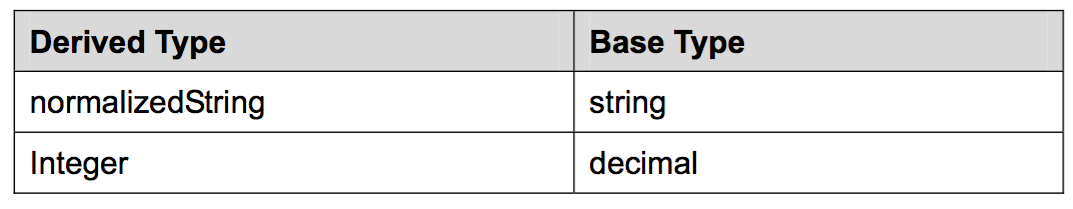
\includegraphics[width=.95\textwidth]{imgs/DerivedTypeBaseType(2types).png}
	\end{center}

	\begin{center}
		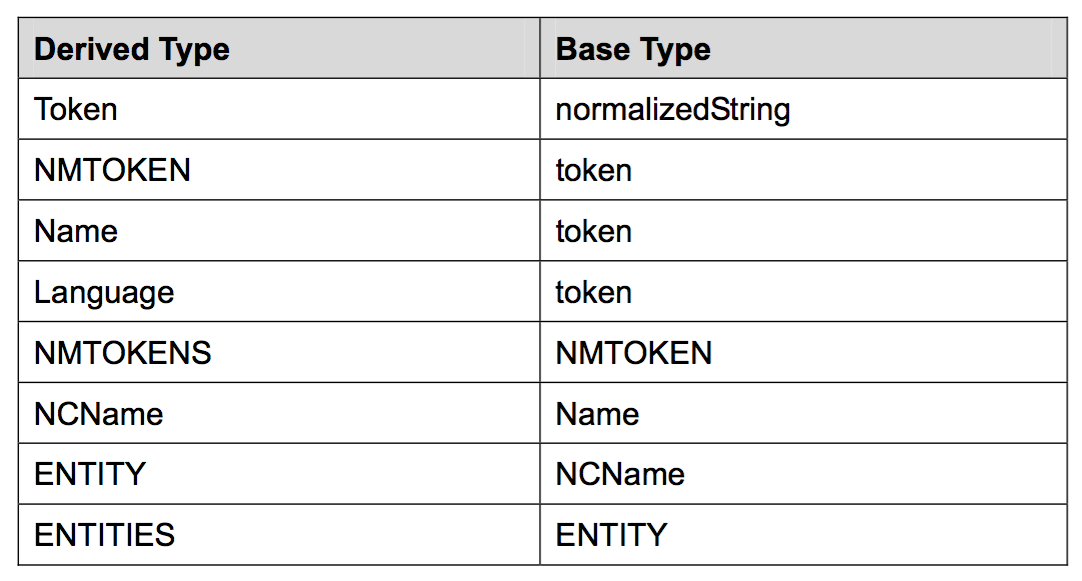
\includegraphics[width=.95\textwidth]{imgs/DerivedTypeFromDerivedType(8types).png}
	\end{center}

\end{frame}

\begin{frame}
	\frametitle{Elementi per la definizione degli schemi xml}
	\framesubtitle{principi XSD}
	\addtocounter{nframe}{1}

	\begin{center}
		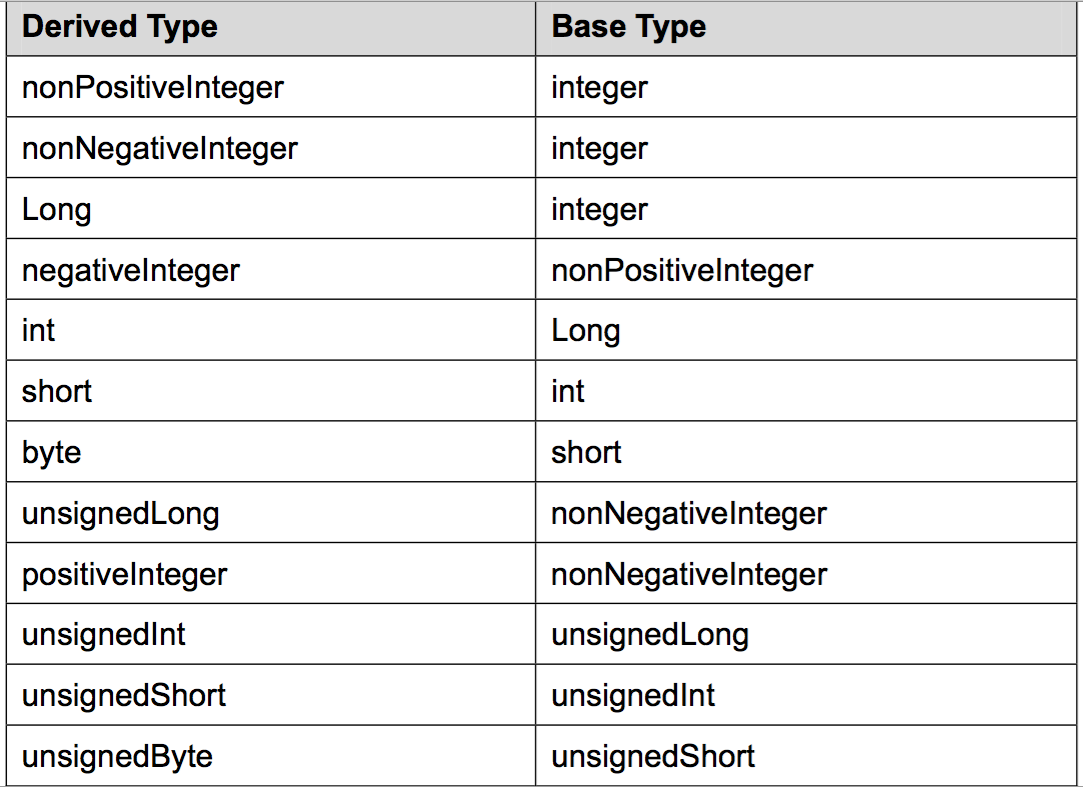
\includegraphics[width=.95\textwidth]{imgs/NumericalDerivedType(12types).png}
	\end{center}

\end{frame}



%% qualche esempio di DataType (libro XSD pagine 175 et seguenti)
% String
% Boolean
% Decimal
%% XSD decimal data type represents a subset of real numbers
% Float
%% XSD float data type is single precision 32-bit floating point type
% Double
%% XSD double data type shares the same characteristics as float except that double data type is double precision 64-bit floating point type.
% Duration
%% XSD duration data type represents duration of time
%% A duration value should always start with the letter "P" in upper case. Then each value should be separated by indicators Y (Years), M (Months), D (Days), H (Hours), M (Minutes) and S (Seconds). Letter "T" should appear as a separator between Year-Month-Day and Hour-Minute-Second.
%% esempio:
% <ElapsedTime>PT3M15S</ElapsedTime>
% DataTime
%% The format of XSD dateTime is -yyyy-mm-ddThh:mm:ss.sZ. 
% hexBinary
%% XSD hexBinary data type represents HEX encoded data.
% "This is a secret message" using the online Text-to- Hex tool available at http://tools.elitehackers.info/Hex.php.
% base64Binary
%% XSD base64Binary data type represents base64 encoded data. store binary data
%% esempio https://www.base64decode.org/
%% VGhpcyBpcyBhIHNlY3JldCBtZXNzYWdl
% QName
%% QName data type can accept a colonized value (a namespace prefix and a string value separated by a colon) only if there is a valid namespace declaration within the scope where the value is used.



\begin{frame}
	\frametitle{Elementi per la definizione degli schemi xml}
	\framesubtitle{principi XSD}
	\addtocounter{nframe}{1}

	\begin{block}{Data Type: Facets}
		Each data type has a number of properties that can be restricted to perform additional validations on the value.
		\\These properties are called \textbf{Facets} in XSD.
	\end{block}

	\begin{block}{Data Type: Facets}
		So each data type has a certain number of predefined Facets.
		\\A facet controls a certain attribute or characteristic of a data type
	\end{block}

\end{frame}

\begin{frame}
	\frametitle{Elementi per la definizione degli schemi xml}
	\framesubtitle{principi XSD}
	\addtocounter{nframe}{1}

	\begin{block}{Data Type: Facets Esempio}
		\texttt{
			<xsd:schema xmlns:xsd=``http://www.w3.org/2001/XMLSchema''>
			<xsd:element name=``name''>
			<xsd:complexType>
			<xsd:attribute name=``type''>
			<xsd:simpleType>
			<xsd:restriction base=``xsd:string''>
			<xsd:length value=``15''/>
			</xsd:restriction>
			</xsd:simpleType>
			</xsd:attribute>
			</xsd:complexType>
			</xsd:element>
			</xsd:schema>
		}

	\end{block}

\end{frame}

\begin{frame}
	\frametitle{Elementi per la definizione degli schemi xml}
	\framesubtitle{principi XSD}
	\addtocounter{nframe}{1}

	\begin{block}{Data Type: Facets Esempio}
		\texttt{
		<xsd:schema xmlns:xsd=``http://www.w3.org/2001/XMLSchema''>
		<xsd:element name=``name''>
		<xsd:complexType>
		<xsd:attribute name=``type''>
		<xsd:simpleType>
		<xsd:restriction base=``xsd:string''>
		<xsd:patter value=``[A-Za-z]+''/>
		</xsd:restriction>
		</xsd:simpleType>
		</xsd:attribute>
		</xsd:complexType>
		</xsd:element>
		</xsd:schema>
		}

	\end{block}

\end{frame}

\begin{frame}
	\frametitle{Elementi per la definizione degli schemi xml}
	\framesubtitle{principi XSD}
	\addtocounter{nframe}{1}

	\begin{center}
		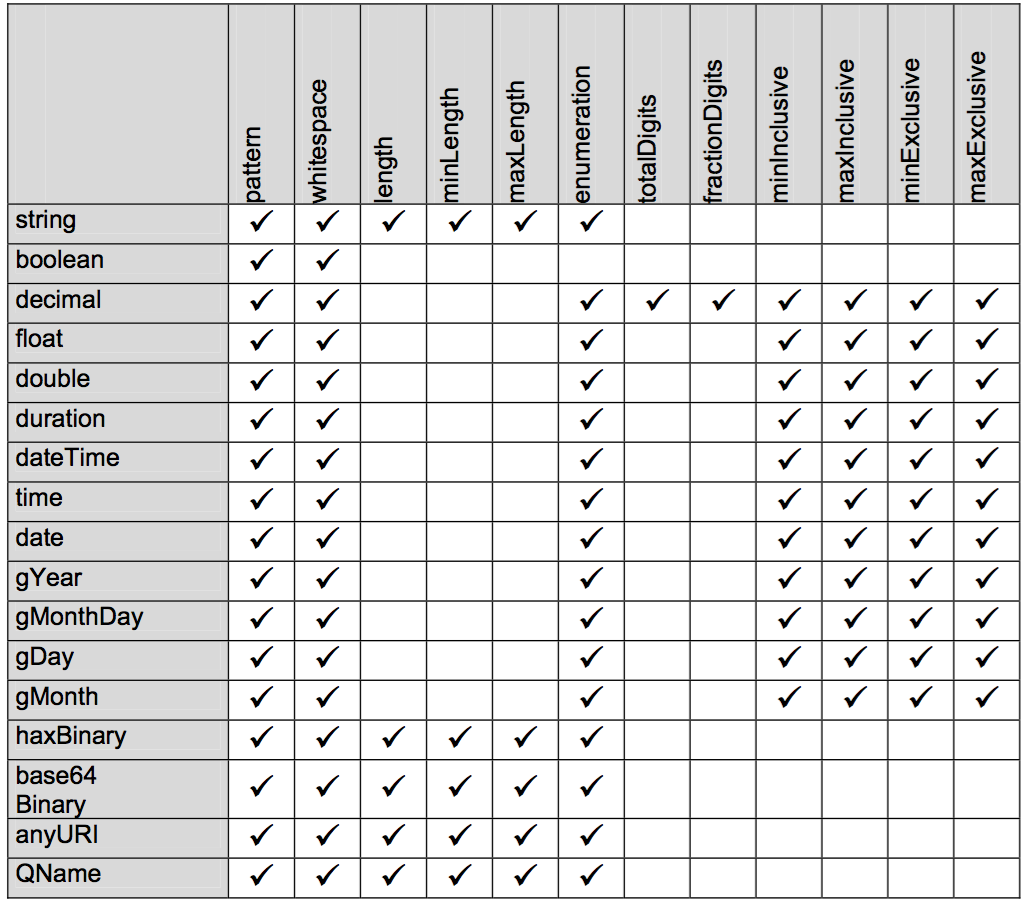
\includegraphics[width=.8\textwidth]{imgs/SchemaDataTypeFacets.png}
	\end{center}

\end{frame}


\begin{frame}
	\frametitle{Elementi per la definizione degli schemi xml}
	\framesubtitle{principi XSD}
	\addtocounter{nframe}{1}

	\begin{block}{Simple Type vs Complex Type}

		The basic distinction between simple types and complex types is that only a complex type can contain child elements and attributes.

	\end{block}

	\begin{block}{Simple Type vs Complex Type}

		Simple types can only store a value. An element or attribute can have a simple type.

	\end{block}

\end{frame}


% Simple types can only store a value. An element or attribute can have a simple type.
% Simple Types can be declared globally or locally. When a simple type is declared globally, it must always have a name.
% When a Simple Type is declared within the scope of an element or attribute it is a local declaration.
%% esempio (simpleTypeGlobalLocal)

\begin{frame}
	\frametitle{Elementi per la definizione degli schemi xml}
	\framesubtitle{principi XSD}
	\addtocounter{nframe}{1}

	\begin{center}
		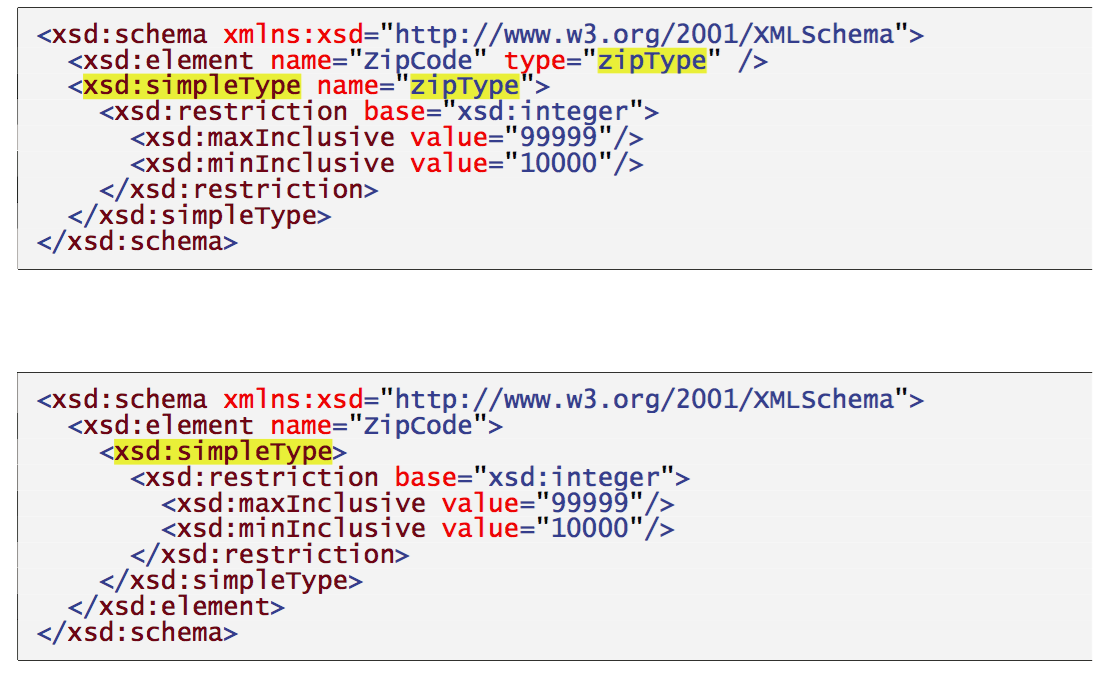
\includegraphics[width=.95\textwidth]{imgs/SimpleTypeGlobalLocal.png}
	\end{center}

	\textit{Simple Types can be declared globally or locally}

\end{frame}


\begin{frame}
	\frametitle{Elementi per la definizione degli schemi xml}
	\framesubtitle{principi XSD}
	\addtocounter{nframe}{1}

	\begin{block}{Global simple types}
		Global simple types help reuse the definitions as well as help organize and maintain the schema.
	\end{block}

	\textit{helpful when the same set of validations is to be performed}

\end{frame}


\begin{frame}
	\frametitle{Elementi per la definizione degli schemi xml}
	\framesubtitle{principi XSD}
	\addtocounter{nframe}{1}

	\begin{block}{simple types example}
		\texttt{
			<xsd:simpleType name=``chapterNumberType''>
			<xsd:restriction base=``xsd:integer''>
			<xsd:maxInclusive value=``1000''/>
			<xsd:minInclusive value=``1''/>
			</xsd:restriction>
			</xsd:simpleType>
		}
	\end{block}

	\begin{block}{simple types example}
		\texttt{
			<xsd:element name=``item''>
			<xsd:complexType>
			<xsd:attribute name=``originalChapter'' type=``chapterNumberType''/>
			</xsd:complexType>
			</xsd:element>
		}
	\end{block}
\end{frame}


% Deriving:
\begin{frame}
	\frametitle{Elementi per la definizione degli schemi xml}
	\framesubtitle{principi XSD}
	\addtocounter{nframe}{1}

	\begin{block}{simple types: deriving}
		Un nuovo tipo può essere derivato da un tipo già dichiarato (primitivo o meno) ed ereditarne le caratteristiche.
	\end{block}

	\begin{block}{simple types example}
		\begin{itemize}
			\item Derive by restriction
			\item Derive by list
			\item Derive by Union
		\end{itemize}
	\end{block}

\end{frame}

\begin{frame}
	\frametitle{Elementi per la definizione degli schemi xml}
	\framesubtitle{principi XSD}
	\addtocounter{nframe}{1}

	\begin{block}{simple types: deriving}
		This involves identifying a base type that is close to what we are looking for, and adding the additional restrictions or validation rules.
	\end{block}

\end{frame}

\begin{frame}
	\frametitle{Elementi per la definizione degli schemi xml}
	\framesubtitle{principi XSD}
	\addtocounter{nframe}{1}

	\begin{block}{simple types: deriving by Restriction}
		A restriction is defined by adding ``xsd:restriction'' to the Simple Type declaration. Each data type has a number of properties that restricts the set of values it can accept (facets). When you derive a new data type by restriction, you restrict one or more facets.
	\end{block}

\end{frame}

\begin{frame}
	\frametitle{Elementi per la definizione degli schemi xml}
	\framesubtitle{principi XSD}
	\addtocounter{nframe}{1}

	\begin{block}{simple types: deriving by Restriction}
		\texttt{
			<xsd:simpleType name=``signatureType''>
			\textit{<xsd:restriction base=``xsd:integer''>}
			\textit{<xsd:totalDigits value=``5''/>}
			</xsd:restriction>
			</xsd:simpleType>
		}
	\end{block}

	\begin{block}{simple types: deriving by Restriction}
		\texttt{
			<xsd:element name=``signature'' type=``signatureType''>
		}
		\texttt{
			<signature>12345</sgnature>
		} \textit{(valido)}
		\texttt{
			<signature>123ab</signature>
		} \textit{(non valido)}
	\end{block}
\end{frame}

% Another way of creating a new Simple Type is by deriving by List: 

\begin{frame}
	\frametitle{Elementi per la definizione degli schemi xml}
	\framesubtitle{principi XSD}
	\addtocounter{nframe}{1}

	\begin{block}{simple types: deriving by List}
		data type can store a SPACE separated list of values accepted by the base type
	\end{block}

	\begin{block}{simple types: deriving by List}
		\texttt{<xsd:simpleType name=``chapterNumberList''>
			<xsd:list itemType=``xsd:integer'' />
			</xsd:simpleType>}
		\\\texttt{
			<xsd:element name=``chapters'' type=``chapterNumberList'' />}
		\\\texttt{
			<chapters>1 53 60 61 205 409</chapters>}
	\end{block}

\end{frame}

\begin{frame}
	\frametitle{Elementi per la definizione degli schemi xml}
	\framesubtitle{principi XSD}
	\addtocounter{nframe}{1}

	\begin{block}{simple types: deriving by Union}
		The derived type can store the values acceptable to any of the base types from which the new type is derived.
	\end{block}

	\begin{block}{simple types: deriving by Union}
		\texttt{<xsd:simpleType name=``ZipCityUnion''>
		  <xsd:union>
		    <xsd:simpleType>
		      <xsd:restriction base="ZipType"/>
		    </xsd:simpleType>
		    <xsd:simpleType>
		      <xsd:restriction base="CityType"/>
		    </xsd:simpleType>
		  </xsd:union>
		 </xsd:simpleType>}
		
	\end{block}

\end{frame}



% A third method of deriving a simple type is by union. The derived type can store the values acceptable to any of the base types from which the new type is derived.
% esempio:

% <xsd:simpleType name="ZipCityUnion">
%  <xsd:union>
%    <xsd:simpleType>
%      <xsd:restriction base="ZipType"/>
%    </xsd:simpleType>
%    <xsd:simpleType>
%      <xsd:restriction base="CityType"/>
%    </xsd:simpleType>
%  </xsd:union>
% </xsd:simpleType>

% The value will be accepted only if it validates successfully with one of the base types.

% It is not allowed to make the value space of a derived type less restrictive than the base type.

\begin{frame}
	\frametitle{Elementi per la definizione degli schemi xml}
	\framesubtitle{principi XSD}
	\addtocounter{nframe}{1}

	\begin{block}{simple types: deriving}
		 The value will be accepted only if it validates successfully with one of the base types.
	\end{block}

	\begin{block}{simple types: deriving}
		It is not allowed to make the value space of a derived type less restrictive than the base type.
	\end{block}

\end{frame}


% each XSD data type has a certain number of facets that control its value space.
% When we derive a new Simple Type from another, the new type will inherit all the facets of the base type. You can set the "fixed" attribute of the given facets to "true" to make sure that the derived types do not modify those facets.

\begin{frame}
	\frametitle{Elementi per la definizione degli schemi xml}
	\framesubtitle{principi XSD}
	\addtocounter{nframe}{1}

	\begin{block}{simple types: deriving facets}
		each XSD data type has a certain number of facets that control its value space.
		\\When we derive a new Simple Type from another, the new type will inherit all the facets of the base type.
	\end{block}

	\begin{block}{simple types: deriving facets}
		You can set the \textbf{fixed} attribute of the given facets to \textbf{true} to make sure that the derived types do not modify those facets.
	\end{block}

\end{frame}


\begin{frame}
	\frametitle{Elementi per la definizione degli schemi xml}
	\framesubtitle{principi XSD}
	\addtocounter{nframe}{1}

	\begin{block}{Simple types: controllare la derivazione}
		XSD provides a way to protect your Simple Type so that no other Types can inherit from it.
		
	\end{block}

	\begin{block}{controllare la derivazione: l'attributo final}
		\begin{itemize}
			\item restriction
			\item list
			\item union
			\item extension
			\item \#all
		\end{itemize}
	\end{block}

\end{frame}


\begin{frame}
	\frametitle{Elementi per la definizione degli schemi xml}
	\framesubtitle{principi XSD}
	\addtocounter{nframe}{1}

	\begin{block}{Simple types: controllare la derivazione - esempio}
		\texttt{
			<xsd:schema xmlns:xsd=``http://www.w3.org/2001/XMLSchema''>
			<xsd:simpleType name=``zipType''
			final=``restriction union list extension''>
			<xsd:restriction base=``xsd:integer''>
			<xsd:maxInclusive value=``99999'' fixed=``true''/>
			<xsd:minInclusive value=``10000''/>
			</xsd:restriction>
			</xsd:simpleType>
			</xsd:schema>
		}
	\end{block}

\end{frame}

\begin{frame}
	\frametitle{Elementi per la definizione degli schemi xml}
	\framesubtitle{principi XSD}
	\addtocounter{nframe}{1}

	\begin{block}{Simple types: controllare la derivazione - esempio}
		Extension refers to deriving a new type from a Simple Type that results in a Complex Type
	\end{block}

	\begin{block}{Simple types: controllare la derivazione - esempio}
		When the \textbf{final} attribute is set to \textbf{\#all}, the Simple Type cannot be inherited at all.
	\end{block}

\end{frame}


% Defining Enumerations
% Sometimes we will come across requirements where we need to apply a certain restriction to an element or attribute so that only a set of predefined values can be stored. 

% XSD Built-in Data Types: Primitive and Derived Data Types
% Facets of built-in data types
% XSD Built-in Derived data types
%% XSD has twenty-five such data types that derive directly or indirectly from one of the Primitive Data types
% xsd:integer is derived from xsd:decimal by restriction
% esempio

%<xs:simpleType name="integer" id="integer">
%  <xs:annotation>
%     <xs:documentation
%       source="http://www.w3.org/TR/xmlschema-2/#integer"/>
%   </xs:annotation>
%   <xs:restriction base="xs:decimal">
%     <xs:fractionDigits fixed="true" value="0"
%                        id="integer.fractionDigits"/>
%     <xs:pattern value="[\-+]?[0-9]+"/>
%   </xs:restriction>
%  </xs:simpleType>

% fractionDigits is a facet exposed by all numeric data types and it restricts the number of decimal places in the value. 
% The attribute fixed indicates that any type that derives from integer is not allowed to modify the value of fractionDigits facet.
% It applies a pattern restriction to validate the format of the value.
% as with integer, each of the XSD built-in derived data types derives from one of the Primitive Types directly or indirectly.

% Facets of Data Types
%% Each data type has a certain set of characteristics that can be used to perform additional validations on the value. Each of the XSD data types has a certain number of such properties that add additional restrictions on the value. These properties are called facets in XSD. Not all data types support the same facets.

% list of all the facets supported by the different data types of XSD.
% length restricts the number of characters a value can accept.
% minLength defines the minimum length of the value
% maxLength defines the maximum length of the value
% pattern specifies a Regular Expression to validate the value.
% enumeration is used to restrict the values to a set of predefined choices
% whitespace defines the way whitespaces is processed by the schema processor (Preserve, replace, collapse).
% totalDigits restricts the number of digits the type can hold (cifre intere + decimali)
% fractionDigits restricts the number of digits in the decimal part of the value
% maxInclusive specifies the highest value the type can accept
% minInclusive specifies the highest numeric value the type can accept, excluding the value specified in the restriction.
% maxExclusive defines the lowest value that the type can accept.
% minExclusive defines the minimum value that the type can accept, excluding the value specified in the restriction

%% foto della tabella (schemaDatatypeFacets)

%% Tipi di dati xsd derivati da tipi di dati primitivi (25 in totale)
%% immagini per i tipi e esempi di catena di derivazione (DerivedTypeBaseType, DerivedTypeFromDerivedType, NumericalDerivedType, NumericalGrafico, String-Grafico).








%% ComplexType
% A complex type can have child elements and/or attributes.
% an element has a Simple Type, it cannot have child elements or attributes. It can store only a text value.
% Attribute declarations cannot have Complex Types
% All global declarations should have a name. A Named Complex Type can be used within the declaration of other complex types.
%% Esempio:

%<xsd:schema xmlns:xsd="http://www.w3.org/2001/XMLSchema">
% <!-- Address Type -->
%  <xsd:complexType name="AddressType">
%     <xsd:all>
%       <xsd:element name="Address"/>
%       <xsd:element name="Street"/>
%       <xsd:element name="City"/>
%       <xsd:element name="Zip"/>
%       <xsd:element name="State"/>
%     </xsd:all>
%   </xsd:complexType>
%   <!-- Customer Information -->
%   <xsd:element name="Customer">
%     <xsd:complexType>
%       <xsd:sequence>
%         <xsd:element name="CustomerName"/>
%         <xsd:element name="Address" type="AddressType"/>
%       </xsd:sequence>
%     </xsd:complexType>
%   </xsd:element>
% </xsd:schema>

% Named Complex Types provide a great deal of reusability.
% Anonymous types appears within the complex type that owns the element.
%% esempio
% <xsd:schema xmlns:xsd="http://www.w3.org/2001/XMLSchema">
%   <!-- Customer Information -->
%   <xsd:element name="Customer">
%     <xsd:complexType>
%       <xsd:sequence>
%         <xsd:element name="CustomerName"/>
%         <xsd:element name="Address">
%           <xsd:complexType>
%             <xsd:all>
%               <xsd:element name="Address"/>
%               <xsd:element name="Street"/>
%               <xsd:element name="City"/>
%               <xsd:element name="Zip"/>
%               <xsd:element name="State"/>
%             </xsd:all>
%           </xsd:complexType>
%         </xsd:element>
%       </xsd:sequence>
%     </xsd:complexType>
%   </xsd:element>
% </xsd:schema>

% Such declarations cannot be reused

%% The structure of the child elements of a Complex Type is called its Content Model.
% Elements having Simple Content can store a text value and can hold attributes.
% When an element has Complex Content, it can be either empty, element- only or mixed type.
% Empty content element may have attributes.
% An element is said to have element-only content when it has child elements – and optionally attributes, too – but doesn't hold a text value.
% When an element has mixed content model it can store child elements, attributes and text value.
% Esempio:
% <Email Priority="High">
%   Dear <name>Jacob</name>,
%   Your order has been
%   shipped on <date>2008-01-01</date>
% </Email>

%% Simple Content
% when an element has Simple Content it can store a text value and can have attributes.
% Simple Content does not allow child elements
%% Esempio:
%<xsd:schema xmlns:xsd="http://www.w3.org/2001/XMLSchema">
%  <xsd:element name="Phone">
%     <xsd:complexType>
%       <xsd:simpleContent>
%         <xsd:extension base="xsd:string">
%           <xsd:attribute name="location" type="xsd:string"/>
%         </xsd:extension>
%       </xsd:simpleContent>
%     </xsd:complexType>
%   </xsd:element>
% </xsd:schema>

% New Complex Types can be derived from Complex Types having Simple Content. It is not allowed to derive Complex Content from Simple Content.

%% Complex Content can store child elements and attributes as well as text values.

%% Empty content
% Complex Types having empty content are very close to the ones having simple content, but they cannot store a text value. However, it can have attributes.
%% Element-only content
% These are Complex Types that hold elements and/or attributes, but no text values.

%% Mixed Content
% Mixed Content is a combination of Simple Content and Element-only content.
% It can store child elements and attributes as well as text values.
% Mixed content type makes text values more meaningful. The Mixed content type XML is more meaningful to an XML parser then simple text, because the information can be extracted more accurately from it. 
% how to write the schema for a Complex Type that has Mixed Content.
%% Esempio
% <xsd:schema xmlns:xsd="http://www.w3.org/2001/XMLSchema">
%   <xsd:element name="InvoiceNote">
%     <xsd:complexType mixed="true">
%       <xsd:sequence>
%         <xsd:element name="name"/>
%         <xsd:element name="mobile"/>
%       </xsd:sequence>
%     </xsd:complexType>
%   </xsd:element>
% </xsd:schema>

% The only difference from element-only content model is the presence of the attribute "mixed." In DSE there are many cases where we would come across mixed types.
% When a Complex Type contains elements and attributes, the attribute declarations should appear after the element declarations.
%% esempio:

% <xsd:schema xmlns:xsd="http://www.w3.org/2001/XMLSchema">
%   <xsd:element name="Customer">
%     <xsd:complexType>
%       <xsd:sequence>
%         <xsd:element name="name"/>
%         <xsd:element name="phone"/>
%       </xsd:sequence>
%       <xsd:attribute name="CustomerNumber"/>
%     </xsd:complexType>
%   </xsd:element>
% </xsd:schema>

% Attribute declarations should always appear after element declarations.
% Attributes of an element can appear in any order. The order/position is not significant for attributes.
% The order/position of elements is significant in XML: specify for each Complex Type whether the children should follow a specific order or not.
% XSD uses order indicators to specify the order in which elements should appear inside an XML node.
% XSD defines the following order indicators:
% - sequence: is used to specify that the elements should appear in exactly the same order as they are defined in the schema (<xsd:sequence />).
% - all: is used to specify that the child elements can appear in any order (<xsd:all>). 
% - choice: is used when only one element from a list of child elements should appear in the XML instance (<xsd:choice />).

%% Occurrence Indicator
% One of the basic differences between an element and attribute is that an element can appear more than once. Attributes cannot appear more than once within the parent element.
% We can control the occurrence of elements by using minOccurs and maxOccurs attributes of element declaration. 
% esempio: The following table shows a few examples that demonstrate how to control the occurrences of elements by using minOccurs and maxOccurs.
% (immagine:TabellaMinMaxOccurs).

%% Element Groups
% provide reusability to a certain extent as they can be inserted into other complex types within the same schema. The schema is easier to modify and maintain.
%% esemipio:
%<xsd:schema xmlns:xsd="http://www.w3.org/2001/XMLSchema">
%   <xsd:group name="ContactInfo">
%     <xsd:sequence>
%       <xsd:element name="email"/>
%       <xsd:element name="phone"/>
%     </xsd:sequence>
%   </xsd:group>
%   <xsd:element name="author">
%     <xsd:complexType>
%       <xsd:sequence>
%         <xsd:group ref="ContactInfo"/>
%       </xsd:sequence>
%    </xsd:complexType>
%   </xsd:element>
% </xsd:schema>
% Una possibile istanza di documento XML validata dallo schema di cui sopra:
% <author>
%       <email>name@institution.it</email>
%       <phone>0039123456789</phone>
% </author>

% Complex Type derivation
% as we saw with simple types, new types can be derived from complex types. New complex types can be derived from existing complex types by restriction or by extension.
% New complex types can be derived from existing complex types by restriction or by extension. When you derive a complex type from a simple type, it can only have a simple content.
% Esempio:
% <xsd:complexType name="PhoneTypeEx">
%   <xsd:simpleContent>
%     <xsd:extension base="PhoneType">
%       <xsd:attribute name="Type" use="required"/>
%     </xsd:extension>
%   </xsd:simpleContent>
% </xsd:complexType>

% When the final attribute is set to "extension," the simple type cannot be extended.
% The derivation behavior of each content model is slightly different from others.
% We can derive a new type by restriction or by extension from complex type simple content model.
%% derive by restriction from a complex type having simple content
% add restrictions to the content/text-value of the element
% add restrictions to the attributes
% remove one or more of the attributes.
%% Esempio:

%<!-- Phone Type -->
%   <xsd:complexType name="PhoneType">
%     <xsd:simpleContent>
%       <xsd:extension base="xsd:string">
%         <xsd:attribute name="Type" type="xsd:string"/>
%         <xsd:attribute name="CallOnWeekend" type="xsd:boolean"/>
%       </xsd:extension>
%     </xsd:simpleContent>
%   </xsd:complexType>
% </xsd:schema>

% <xsd:complexType name="RestrictedPhoneType">
%   <xsd:simpleContent>
%     <xsd:restriction base="PhoneType">
%       <xsd:pattern value="[0-9]{3}-[0-9]{3}-[0-9]{4}"/>
%       <xsd:attribute name="Type">
%         <xsd:simpleType>
%           <xsd:restriction base="xsd:string">
%           <xsd:enumeration value="Home"/>
%             <xsd:enumeration value="Work"/>
%           </xsd:restriction>
%         </xsd:simpleType>
%       </xsd:attribute>
%       <xsd:attribute name="CallOnWeekend" type="xsd:boolean" use="prohibited"/> 
%     </xsd:restriction>
%   </xsd:simpleContent>
% </xsd:complexType>
%% Note the usage of "prohibited." If you want to eliminate one or more attributes, you need to redefine them in the child type and set the "use" attribute to "prohibited."
% Note that when you add restrictions to the content as well as attributes, you cannot make the values less restrictive. Similarly, if an attribute is "required" in the base type, you cannot make it "optional" in the derived type.

%% When you derive by extension from a complex type with simple content the result will always be a simple content. The only operation you can do when you extend a simple content type is to add new attributes.
%% esempio:
% <xsd:complexType name="ExtendedPhoneType">
%   <xsd:simpleContent>
%     <xsd:extension base="PhoneType">
%       <xsd:attribute name="CallOnHolidays" type="xsd:string"/>
%     </xsd:extension>
%   </xsd:simpleContent>
% </xsd:complexType>

%% A complex type with element-only content can be extended or restricted to create new types. The most common usage of deriving by restriction from an element-only content type is to remove one or more elements or attributes. Elements from the base type are not passed down to the derived type by default. 
% All mandatory elements in the base type must exist in the derived type as well. 
%% If the elements in the base type are declared within a sequence group, the derived type cannot change it to all or choice groups. 
%% If the base type has all, the derived type can change it to sequence. 
%% If the base type has choice, the derived type must also have choice.
% All attributes of the base type are passed down to the derived type by default.
% if you want to remove an attribute you need to re-declare it in the derived type as "prohibited."
% A derived type cannot eliminate an attribute declared as mandatory in the base type.
% You need to redefine an attribute in the derived type only if you want to restrict the value space of the attribute.
% Esempio:

% <xsd:schema xmlns:xsd="http://www.w3.org/2001/XMLSchema">
%   <!-- Contact Element -->
%   <xsd:element name="Contact" type="RestrictedContactType"/>

%   <!-- Contact Type -->
%   <xsd:complexType name="ContactType">
%     <xsd:sequence>
%       <xsd:element name="Phone" minOccurs="0"/>
%       <xsd:element name="Email" minOccurs="0"/>
%     </xsd:sequence>
%     <xsd:attribute name="Name" />
%     <xsd:attribute name="Title"/>
%   </xsd:complexType>
%
%
%   <!-- Restricted Contact Type -->
%   <xsd:complexType name="RestrictedContactType">
%     <xsd:complexContent>
%       <xsd:restriction base="ContactType">
%         <xsd:sequence>
%           <xsd:element name="Phone">
%             <xsd:simpleType>
%               <xsd:restriction base="xsd:string">
%                 <xsd:pattern value="[0-9]{3}-[0-9]{3}-[0-9]{4}"/>
%               </xsd:restriction>
%             </xsd:simpleType>
%            </xsd:element>
%          </xsd:sequence>
%         <xsd:attribute name="Title" use="prohibited"/>
%         <xsd:attribute name="Name">
%           <xsd:simpleType>
%             <xsd:restriction base="xsd:string">
%               <xsd:maxLength value="20"/>
%             </xsd:restriction>
%           </xsd:simpleType>
%         </xsd:attribute>
%       </xsd:restriction>
%     </xsd:complexContent>
%   </xsd:complexType>
% </xsd:schema>

% It is also possible to derive an empty content complex type from an element-only content type. By keeping the restriction element empty, we can derive an empty content type. This does not affect the attributes. 
% Gli elementi del tipo dell'elemento base devono essere opzionali.

%% complex types are extended to add new elements and attributes. When deriving by extension, all elements and attributes in the base type will be passed down to the derived type by default.
%% Esempio:

% <xsd:schema xmlns:xsd="http://www.w3.org/2001/XMLSchema">
%   <!-- Contact Element -->
%   <xsd:element name="Contact" type="ExtendedContactType"/>
%   
%   <!-- Extended Contact Type -->
%   <xsd:complexType name="ExtendedContactType">
%     <xsd:complexContent>
%       <xsd:extension base="ContactType">
%         <xsd:sequence>
%           <xsd:element name="Fax"/>
%         </xsd:sequence>
%         <xsd:attribute name="Department"/>
%       </xsd:extension>
%     </xsd:complexContent>
%   </xsd:complexType>
%  
%    <!-- Contact Type -->
%   <xsd:complexType name="ContactType">
%     <xsd:sequence>
%       <xsd:element name="Phone"/>
%       <xsd:element name="Email" minOccurs="0"/>
%     </xsd:sequence>
%     <xsd:attribute name="Name" use="required"/>
%     <xsd:attribute name="Title"/>
%   </xsd:complexType>
% </xsd:schema>
%
%% Una possibile istanza XML:
% <Contact Name="Jacob" Title="Manager" Department="IT">
%   <Phone>999-888-7777</Phone>
%   <Email>jacob@jacob.com</Email>
%   <Fax>888-999-3333</Fax>
% </Contact>

%% You can derive new complex types from a mixed content complex type by restriction or by extension. Derivation of complex types with mixed content is very similar to the derivation of element-only types.
%  when deriving by restriction from a mixed type, you can derive a mixed type, element-only type or empty content type. The rules of derivation are similar to the rules of element-only content model: Elements declared in the parent type do not pass down to the derived type.
% esempio:
% <xsd:complexType name="RestrictedNoteType" mixed="true">
%     <xsd:complexContent>
%       <xsd:restriction base="NoteType">
%         <xsd:sequence>
%           <xsd:element name="name"/>
%         </xsd:sequence>
%       </xsd:restriction>
%     </xsd:complexContent>
%   </xsd:complexType>
% 
% by simply removing the "mixed" attribute from the complex type declaration you derive an element-only complex type from mixed content.

%% When deriving from a mixed type by restriction, we could create an empty content type if all the elements in the base type are optional. By keeping the restriction element empty we could eliminate all the elements declared in the base type (if those elements are declared optional in the base type). To eliminate attributes, you need to declare them in the derived type with prohibited attribute.

% the XSD specification allows deriving a simple content from a mixed-content type,
% esempio:
% <xsd:complexType name="SimpleNoteType">
%     <xsd:simpleContent>
%       <xsd:restriction base="NoteType">
%         <xsd:simpleType>
%           <xsd:restriction base="xsd:string"/>
%         </xsd:simpleType>
%       </xsd:restriction>
%     </xsd:simpleContent>
%   </xsd:complexType>

%% when deriving by extension, we could create only a mixed content complex type.
% esempio:
% <xsd:schema xmlns:xsd="http://www.w3.org/2001/XMLSchema">
%   <!-- Invoice Note Element -->
%   <xsd:element name="InvoiceNote" type="ExtendedNoteType"/>
%   <!-- Extended Note Type -->
%   <xsd:complexType name="ExtendedNoteType" mixed="true">
%     <xsd:complexContent>
%       <xsd:extension base="NoteType">
%         <xsd:sequence>
%           <xsd:element name="email"/>
%         </xsd:sequence>
%       </xsd:extension>
%     </xsd:complexContent>
%   </xsd:complexType>
%   <!-- Note Type -->
%   <xsd:complexType name="NoteType" mixed="true">
%     <xsd:sequence>
%       <xsd:element name="name"/>
%       <xsd:element name="mobile"/>
%     </xsd:sequence>
%   </xsd:complexType>
% </xsd:schema>
% Una possibile istanza XML
% <InvoiceNote>
%   Call <name>Steve</name> on <mobile>999 999 9999</mobile> or <email>steve@somedomain.com</email> before shipping the order.
% </InvoiceNote>

% Derive a new type from an empty content element by restriction or by extension.
% Since an empty content complex type can have only attributes, the only purpose of deriving from an empty content type by restriction is to eliminate attributes or add additional validations to the attributes.
%% esempio:
% <xsd:complexType name="RestrictedPhoneType">
%   <xsd:complexContent>
%     <xsd:restriction base="PhoneType">
%       <xsd:attribute name="Work" use="prohibited"/>
%       <xsd:attribute name="Home">
%         <xsd:simpleType>
%           <xsd:restriction base="xsd:string">
%             <xsd:pattern value="[0-9]{3}-[0-9]{3}-[0-9]{4}"/>
%           </xsd:restriction>
%         </xsd:simpleType>
%       </xsd:attribute>
%     </xsd:restriction>
%   </xsd:complexContent>
% </xsd:complexType>

% when you derive by extension you can create an empty type, mixed type or element only content type.
%% when you derive by extension you can create an empty type, mixed type or element only content type.
%% we can derive an element only content type from an empty content type by extension
% esempio:
% <xsd:complexType name="EmptyPhoneType">
%   <xsd:complexContent>
%     <xsd:extension base="PhoneType">
%       <xsd:sequence>
%         <xsd:element name="Mobile"/>
%       </xsd:sequence>
%     </xsd:extension>
%   </xsd:complexContent>
% </xsd:complexType>

%% It is also possible to derive a mixed content type from an empty content type.
% Esempio:
% <xsd:complexType name="EmptyPhoneType" mixed="true">
%   <xsd:complexContent>
%     <xsd:extension base="PhoneType">
%        <xsd:sequence>
%            <xsd:element name="Mobile"/>
%       </xsd:sequence>
%     </xsd:extension>
%   </xsd:complexContent>
% </xsd:complexType>
%% una possibile istanza XML:
% <Phone Home="888-888-8888" Work="777-777-7777">
%   If not available at home or work, call me on my
%   <Mobile>666-666-6666</Mobile>.
% </Phone>
% 
% Per ricapitolare:
% New complex types can be created from complex types by extension and restriction.
% (tabella riepilogativa content type derivation)

% how to control the derivation of a given complex type: The derivation of a complex type can be controlled by using the final attribute of Complex Type Declaration.
% taking one of the following three values:
% restriction: prevent derivation by restriction
% extension: derivation by extension
% #all: prevent type derivation by restriction or by extension
% esempio:
% <xsd:complexType name="ContactType" final="extension restriction">
%   <xsd:sequence>
%     <xsd:element name="Phone" minOccurs="0"/>
%   </xsd:sequence>
%   <xsd:attribute name="Name" />
% </xsd:complexType>

% derivazione invalida:
% <xsd:complexType name="ExtendedContactType">
%     <xsd:complexContent>
%       <xsd:extension base="ContactType"/>
%     </xsd:complexContent>
%   </xsd:complexType>

%